\chapter{Introduction}
% Topic

\section{Motivations}
% Current situations
% Why there needs further research

As the pandemic of COVID-19 spreading throughout the world since 2020,
people were forced or encouraged to stay home and restricted from accessing public places,
including tourist attractions, shops, workplaces, schools, etc.
Humans' freedom in physical space is restricted, which accelerate the progress of digitalization.
Not only entertainment but more and more economic and even academic activities are moving online.
As the pandemic slowing down recently, despite the resumption of some physical activities,
there are places or facilities remaining unused or abandoned due to financial problems,
amount of users not recovered, digitalization of activities, and so on.

Removing the idle places or facilities is a choice, but if it is possible to give them new values or change people's image of them,
they can play different roles and keep contributing the society or enrich the environment.
In fact, the concept 'Regional Revitalization', which referes to the attempts to vitalize rural towns where population is falling,
by making use of local speciality combined with new ideas to develop new and unique industries such as tourism, has been applied around Japan recently.
Among cases of Regional Revitalization, some of them adopt location-based Augmented Reality to help enrich the space.
Location-based Augmented Reality is defined as Augmented Reality that utilize geographical information to display contents corresponding to a physical location.
It has already used in not merely entertainment, where Pokemon GO is a famous example,
but also implemented in tourism and education, which implies its versatility and practicability.
With the application of location-based Augmented Reality and the reference of Regional Revitalization,
transformation of an idle place or facility without physical reconstruction seems to be feasible.

% BUT not all places are tourist attractions; each place has its unique features and original functionalities; customizing contents for each place is difficult
  % -> Common characteristics: People!
  % -> Enable people to create new values / images for the place (co-creation)
% BUT how to encourage people?
  % -> User-user interaction!

\section{Objectives and importance}
% RQ
【RQ】Location-based AR+ユーザ共創のコンテンツが:
ある場所をもっと魅力的にする?
ある場所がユーザにとっての意義が変わる?
ユーザ同士の交流ができている?

% goals
キャンパスの元気を取り戻す and answer the RQs
propose a general model to vitalize an arbitrary place

% hypotheses
significant, positive effect

% importance
* (Preliminary studies of) Local transformation in general, instead of only tourism or education goals
* Use ‘people’ to comprise the contents, instead of considering specific characteristics of each location
* Prove a possibility, instead of focusing on detailed improvement of technology
    * Future work: combined with improved technology

\section{Overview of this paper}
% order of sections in this paper
% outline the methodology

\section{Sample section}

Sample template \cite{alphago}

\begin{figure}
  \centering
  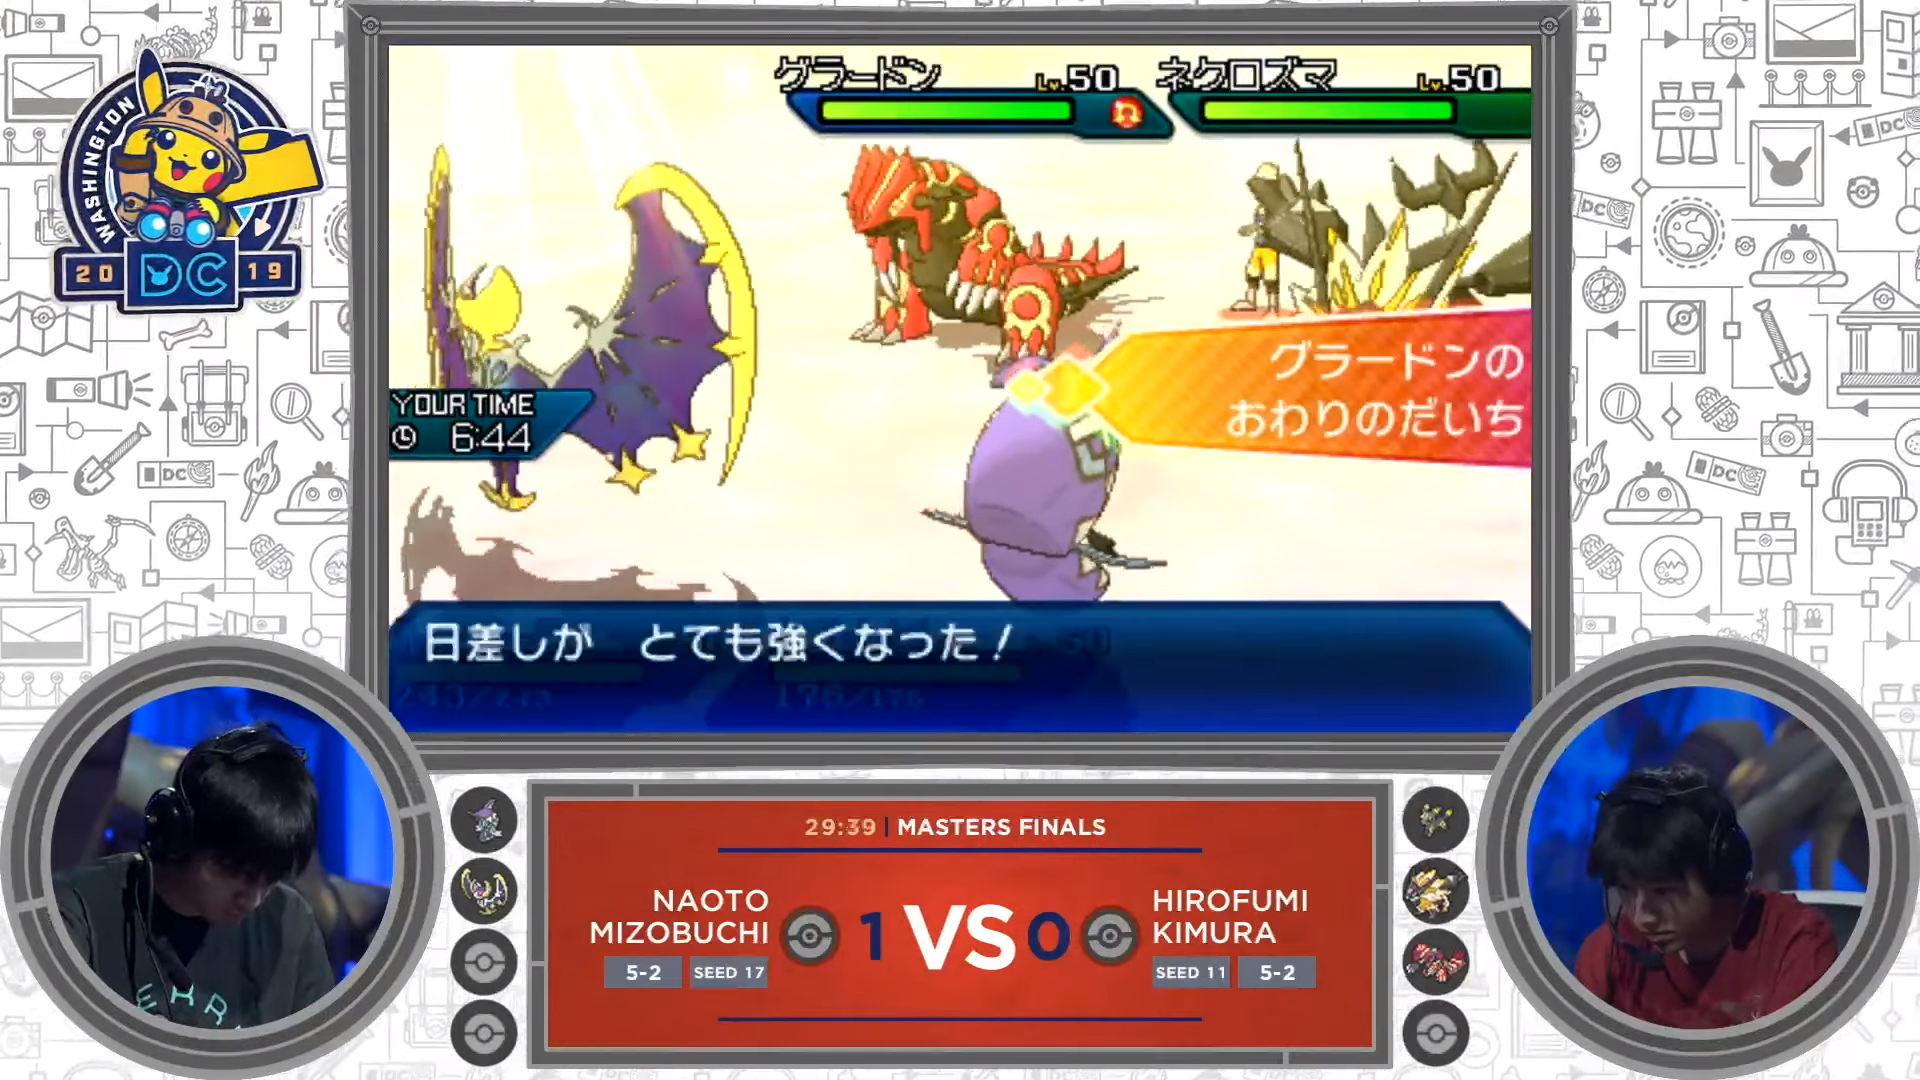
\includegraphics[width=\columnwidth]{resources/1_intro/vgc2019.png}
    \caption{Screenshot of the Grand Finals of the Pokemon Video Game Championships 2019 held in Washinton D.C.}
\end{figure}

